%!TEX TS-program = pdflatex
\documentclass[10pt,wide,xcolor={x11names},hyperref={colorlinks=false},pantone312,mygreen,handout]{beamer}

% Basics und Codierung
% ===========================================================
\usepackage{wwustyle2}
\usepackage[ngerman]{babel}
\usepackage[utf8]{inputenc}
\usepackage[T1]{fontenc}
\usepackage[german=quotes]{csquotes}
\usepackage{scrtime}
\usepackage{etex}
\usepackage{shellesc}
% ===========================================================


% Fonts und Typographie
% ===========================================================
\usepackage{sourcecodepro}
\usepackage[default]{sourcesanspro}
\usepackage{nimbusmononarrow}
\usepackage{ellipsis}
\newcommand{\bet}[1]{\textbf{\color{maincolor}#1}}
\newcommand{\minor}[1]{\textcolor{black!50}{#1}}
\newcommand{\minoritem}{\item[{\footnotesize \textcolor{black!50}{$\blacktriangleright$}}]}
\newcommand{\code}[1]{\texttt{#1}}
\usepackage{xspace}
\makeatletter 
\xspaceaddexceptions{\grqq \grq \csq@qclose@i \} } 
\makeatother
\usefonttheme[onlymath]{serif}
\usepackage{multicol}
% ===========================================================

% Farben	
% ===========================================================
	\usepackage{xcolor}
	\definecolor{fbblau}{HTML}{3078AB}
	\definecolor{mediumgray}{gray}{.65}
	\definecolor{blackberry}{rgb}{0.53, 0.0, 0.25}
% ===========================================================

	
% Mathe-Pakete
% ===========================================================
	\usepackage{mathtools}
	\usepackage{amssymb}
	\usepackage[bigdelims]{newtxmath}

	% Abkürzungen
% ===========================================================
	\newcommand{\BB}{\mathbb{B}}
	\newcommand{\CC}{\mathbb{C}}
	\newcommand{\EE}{\mathbb{E}}
	\newcommand{\FF}{\mathbb{F}}
	\newcommand{\HH}{\mathcal{H}}
	\newcommand{\KK}{\mathbb{K}}
	\newcommand{\LL}{\mathbb{L}}
	\newcommand{\NN}{\mathbb{N}}
	\newcommand{\QQ}{\mathbb{Q}}
	\newcommand{\RR}{\mathbb{R}}
	\newcommand{\ZZ}{\mathbb{Z}}
	\newcommand{\oh}{\mathcal{O}}				% Landau-O
	\newcommand{\ind}{1\hspace{-0,8ex}1} 		% Indikatorfunktion (Doppeleins)
	\newcommand{\bewrueck}{\enquote{$\Leftarrow$}:} 	% Beweis Rückrichtung
	\newcommand{\bewhin}{\enquote{$\Rightarrow$}:}		% Beweis Hinrichtung
	\newcommand{\ol}[1]{\overline{#1}}
	\newcommand{\wt}[1]{\widetilde{#1}}
	\newcommand{\wh}[1]{\widehat{#1}}
% ===========================================================

% Operatoren
% ===========================================================
	\DeclareMathOperator{\id}{id} 				% Identität
	\DeclareMathOperator{\im}{im} 				% image
	\DeclareMathOperator{\pot}{\mathcal{P}}		% Potenzmenge
	\DeclareMathOperator{\sgn}{sgn} 			% Signum
	\DeclareMathOperator{\Sym}{Sym} 			% Symmetrische Gruppe
% ===========================================================

% Klammerungen und ähnliches
% ===========================================================
	\DeclarePairedDelimiter{\absolut}{\lvert}{\rvert}		% Betrag
	\DeclarePairedDelimiter{\ceiling}{\lceil}{\rceil}		% aufrunden
	\DeclarePairedDelimiter{\Floor}{\lfloor}{\rfloor}		% aufrunden
	\DeclarePairedDelimiter{\Norm}{\lVert}{\rVert}			% Norm
	\DeclarePairedDelimiter{\sprod}{\langle}{\rangle}		% spitze Klammern
	\DeclarePairedDelimiter{\enbrace}{(}{)}					% runde Klammern
	\DeclarePairedDelimiter{\benbrace}{\lbrack}{\rbrack}	% eckige Klammern
	\DeclarePairedDelimiter{\penbrace}{\{}{\}}				% geschweifte Klammern
	\newcommand{\Underbrace}[2]{{\underbrace{#1}_{#2}}} 	% bessere Unterklammerungen
	% Kurzschreibweisen für Faule und Code-Vervollständigung
	\newcommand{\abs}[1]{\absolut*{#1}}
	\newcommand{\ceil}[1]{\ceiling*{#1}}
	\newcommand{\flo}[1]{\Floor*{#1}}
	\newcommand{\no}[1]{\Norm*{#1}}
	\newcommand{\sk}[1]{\sprod*{#1}}
	\newcommand{\enb}[1]{\enbrace*{#1}}
	\newcommand{\penb}[1]{\penbrace*{#1}}
	\newcommand{\benb}[1]{\benbrace*{#1}}
% ===========================================================

	\usepackage{wasysym}
	
\newcommand{\zerodisplayskips}{%
%\setlength{\abovedisplayskip}{0pt}%
%\setlength{\belowdisplayskip}{0pt}%
%\setlength{\abovedisplayshortskip}{0pt}%
%\setlength{\belowdisplayshortskip}{0pt}
%\setlength{\multicolsep}{0pt}
}
\appto{\normalsize}{\zerodisplayskips}
\appto{\small}{\zerodisplayskips}
\appto{\footnotesize}{\zerodisplayskips}
% ===========================================================

% TikZ
% ===========================================================
	\usepackage{tikz}
	\usepackage{tikz-cd}					% kommutative Diagramme
	\usetikzlibrary{arrows.meta}			% mehr Pfeile!
	\usetikzlibrary{shadows}
	\usetikzlibrary{calc}
	\tikzset{>=Latex}						% Standard-Pfeilspitze
	\usetikzlibrary{automata,positioning}
	\usetikzlibrary{matrix}
% ===========================================================

% minted
% ===========================================================
\usepackage{minted}
\setminted{%
	style=default,
	fontsize=\footnotesize,
	breaklines,
	breakanywhere=false,
	breakbytoken=false,
	breakbytokenanywhere=false,
	breakafter={.,},
	autogobble,
	numbers=left,
	numbersep=3mm,
	tabsize=4,
	frame=lines
}
\setmintedinline{%
	fontsize=\normalsize,
	numbers=none,
	numbersep=12pt,
	tabsize=4,
	%bgcolor=gray!15,
}
% ===========================================================

\usepackage[%
	backend=biber,
	sortlocale=auto,
	natbib,
	hyperref,
	backref=false,
	style=numeric,
]%
{biblatex}
\addbibresource{bibliography.bib}
\setbeamertemplate{bibliography item}[text]

\hypersetup{citecolor=maincolor}
\author{Phil Steinhorst (\texttt{p.st@wwu.de})}
\title{Informatik I -- Grundlagen der Programmierung}
\subtitle{Einführung in LaTeX}
\date{26. Oktober 2017}
\usepackage{smartdiagram}
\begin{document}
\setbeamertemplate{section in toc}[sections numbered]
\setbeamertemplate{subsection in toc}[subsections numbered]

\begin{frame}[plain]
  \maketitle
\end{frame}

\begin{frame}[t]{Agenda}
\tableofcontents[]
\end{frame}

\AtBeginSection[]
{
	\begin{frame}[t]
		\tableofcontents[currentsection, sectionstyle=show/shaded]
	\end{frame}
}
\AtBeginSubsection[]
{
	\begin{frame}[t]
	\tableofcontents[currentsubsection,sectionstyle=show/shaded,subsectionstyle=show/shaded]
\end{frame}
}

\section{Was ist LaTeX?}
\begin{frame}[t]{\secname}
	\begin{itemize}[<+->]
		\item Textsatzsystem zum Setzen ansprechender Texte mit mathematischen Inhalten.
		\minoritem \minor{Eigentlich: Erweiterung für das Textsatzsystem TeX}
		\item De-facto-Standard in Mathematik, Informatik, Naturwissenschaften und mathematiknahen Disziplinen \cite{CTAN}
		\item frei \cite{LPPL}
	\end{itemize}
\end{frame}

\begin{frame}[t]{Warum LaTeX?}
	LaTeX bietet zahlreiche Vorteile gegenüber gängigen Textverarbeitungsprogrammen: \cite{CTAN}
	\begin{itemize}[<+->]
		\item Klare Trennung von Inhalt und Formatierung
		\item Schnell und stabil -- auch bei komplexen Dokumenten
		\item Einfacheres und mächtigeres Setzen mathematischer Formeln
		\item Plattformunabhängig
		\item Flexibilität -- diese Präsentation wurde mit LaTeX erstellt!
		\item Ausgeprägte Modularität
		\item Automatisiertes Erstellen von Inhaltsverzeichnissen, Abschnittsnummerierungen, Literaturverzeichnissen, \dots
		\item Programmierbar durch Kontrollstrukturen
		\item Zuverlässiges Zitieren und \textit{cross referencing}
		\item Unterstützt Vektorgrafiken
		\item Automatisches Syntax Highlighting
		\item<.-> \dots
	\end{itemize}
\end{frame}

\section{Wie funktioniert das?}
\begin{frame}[t]{TeX-Dateien}
	\begin{itemize}[<+->]
		\item Beim \enquote{TeXen} verfasst man zunächst \bet{Quellcode} in einer simplen Textdatei mit \code{.tex}-Endung:
		\onslide<2->{\inputminted[]{latex}{code/minimal.tex}}
		\item<+(1)-> Ein \bet{Compiler} erzeugt daraus ein gewünschtes Output-Format:	
		\begin{center}
			\code{pdflatex HelloWorld.tex}
		\end{center}
		\begin{center}
			
\includegraphics[keepaspectratio,width=7cm]{img/minimal.pdf}
		\end{center}		
		\item<+(1)-> Standard-Compiler (und empfohlen für PDF-Ausgabe): \bet{\texttt{pdflatex}}
	\end{itemize}
\end{frame}

\begin{frame}[t,fragile]{}
\begin{itemize}[<+->]
	\item Eine TeX-Datei (\code{.tex}) beginnt \minor{in der Regel} mit einer so genannten \bet{Präambel}:
	\inputminted[firstline=1,lastline=10]{latex}{code/preamble.tex}
	\item In dieser werden alle Einstellungen des Dokuments festgelegt, wie z.B. Layout, eigene Befehle und zusätzliche Pakete. \bet{Dies erzeugt noch keinen sichtbaren Output!}
	\item Notwendig: \mintinline{latex}{\documentclass{...}}-Befehl zu Beginn zum Festlegen der Dokumentklasse.
	\begin{itemize}
		\item Empfohlen: \bet{KOMA-Script-Klassen} (\code{scrartcl, scrreprt, scrbook, } \dots) statt der Standardklassen (\code{article, report, book, } \dots)
	\end{itemize}
\end{itemize}
\end{frame}


\begin{frame}[t,fragile]{}
\begin{itemize}[<+->]
	\item Der eigentliche Inhalt, der ausgegeben werden soll, befindet sich in der \code{document}-Umgebung:
	\inputminted[]{latex}{code/preamble.tex}
	\item Text nach \mintinline{latex}{\end{document}} wird nicht verarbeitet.
\end{itemize}
\end{frame}

\begin{frame}[t,fragile]{TeX-Workflow}
	\begin{center}
		\smartdiagram[circular diagram:clockwise]{Quellcode schreiben, kompilieren, Output begutachten}
	\end{center}
\end{frame}

\section{Praktische Hinweise}
\subsection{Mathematische Formeln}
\begin{frame}[t,fragile]{Mathematische Formeln}
Mathematische Formeln können auf verschiedene Arten und Weisen im so genannten \bet{math mode} gesetzt werden:
\begin{itemize}
	\item<2-> Innerhalb von Fließtext (\bet{inline}) mittels \mintinline{latex}{$...$}:
		\begin{description}
			\item<3->[Input:] \mintinline{latex}{Die Formel $a^2 + b^2 = c^2$ steht inline.}
			\item<4->[Output:] Die Formel $a^2 + b^2 = c^2$ steht inline.
		\end{description}
	\item<5-> Das sieht bei in die Höhe wachsenden Formeln unschön aus:
		\begin{description}
			\item<6->[Input:] \mintinline{latex}{Die Formel $x := \frac{1}{1+\frac{1}{1+\frac{1}{2}}}$ sprengt die Zeilenhöhe, was mitten im Fließtext sehr unschön aussieht.}
			\item<7->[Output:] Die Formel $x := \frac{1}{1+\frac{1}{1+\frac{1}{2}}}$ \quad sprengt die Zeilenhöhe, was mitten im Fließtext sehr unschön aussieht.
		\end{description}
\end{itemize}
\end{frame}

\begin{frame}[t]{}
	Besser: Einzeilige Formeln mittels \mintinline{latex}{\[ ... \]} abgesetzt und zentriert darstellen: \pause
	\inputminted[linenos=false]{latex}{code/einzeilig.tex} \pause
	\bet{Output:}
	
	Die Formel
\[ x := \frac{1}{1+\frac{1}{1+\frac{1}{2}}} \]
wird abgesetzt und zentriert dargestellt.
\end{frame}

\begin{frame}[t]{Mehrzeilige Formeln und Rechnungen}
So \bet{nicht}:
\inputminted[linenos=false]{latex}{code/mehrzeilig-falsch.tex} \pause
\bet{Output:}

$f(x)   = x^2 + 2x - 7$ \\
$f'(x)  = 2x+2$ \\
$f''(x) = 2$ \pause

\begin{itemize}
	\item Für mehrzeilige Rechnungen bieten sich Umgebungen wie \mintinline{latex}{align} an.
\end{itemize}
\end{frame}

\begin{frame}[t]{}
\inputminted[linenos=false]{latex}{code/mehrzeilig-richtig.tex} \pause
\bet{Output:}

\vspace*{-0.5cm}

\begin{align}
	f(x) &= x^2 + 2x - 7 \\
	f'(x) &= 2x+2 \\
	f''(x) &= 2
\end{align}

\begin{itemize}
	\item<3-> Zeilen werden so ausgerichtet, dass die \mintinline{latex}{&} untereinander stehen.
	\item<4-> Nummerierung kann mit \mintinline{latex}{\nonumber} pro Zeile ausgeschaltet werden -- oder man nutzt \mintinline{latex}{align*} statt \mintinline{latex}{align}.
	\item<5-> Andere nützliche Umgebungen sind \mintinline{latex}{equation, gather, array}.
	\item<6-> Lieber vermeiden: \mintinline{latex}{eqnarray}-Umgebung \cite{eqnarray}
\end{itemize}
\end{frame}

\begin{frame}[t]{Nummerieren von Formeln}
\begin{itemize}
	\item Das Nummerieren von Formeln hat den Sinn, dass man sich an anderer Stelle auf diese Formel beziehen kann, ohne dass man die Formel erneut aufschreiben muss.
\inputminted[linenos=false]{latex}{code/ref-formel.tex} \pause
\bet{Output:}

\vspace*{-0.5cm}

\begin{align}
	\sum_{i=0}^{n} x^i &= \frac{1-x^{n+1}}{1-x} \label{formel-A} \\
	\sum_{i=0}^{n} \frac{1}{2^i} &= 2 - \frac{1}{2^n} \label{formel-B}
\end{align}

Formel \eqref{formel-B} ist ein Spezialfall von Formel \eqref{formel-A}.
\end{itemize}
\end{frame}

\begin{frame}[t]{Nummerieren von Formeln}
\inputminted[linenos=false]{latex}{code/ref-formel.tex}
\begin{itemize}
	\item Dafür gibt es die Befehle \mintinline{latex}{\label}, um eine Formel zu benennen, und \mintinline{latex}{\eqref}, um sie anhand des vergebenen Namens zu referenzieren.
	\item LaTeX kümmert sich selbst um eine konsistente Nummerierung!
	\item Ähnlich können auch Abschnitte, Tabellen, Abbildungen, \dots \ referenziert werden.
\end{itemize}
\end{frame}

\begin{frame}[t]{Angeben von Funktionen}
\inputminted[linenos=false]{latex}{code/funktion1.tex}
\bet{Output:}

\vspace*{-0.5cm}

\begin{align*}
	f \colon \mathbb{R} &\longrightarrow \mathbb{R} \\
	x &\longmapsto x^2
\end{align*}
\end{frame}

\begin{frame}[t]{Mathematische Symbole}
\begin{itemize}
	\item Falls man einen Befehl für ein bestimmtes mathematisches Symbol sucht, hilft der Dienst \href{http://detexify.kirelabs.org/classify.html}{\bet{Detexify}} weiter: \pause
	\begin{center}
		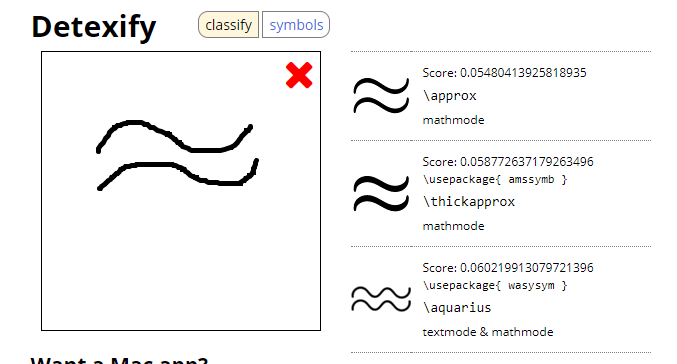
\includegraphics[keepaspectratio,width=8cm]{img/detexify.png}
	\end{center}
\end{itemize}
\end{frame}

\subsection{Listen}
\begin{frame}[t,fragile]{Listen}
\begin{itemize}
	\item Ein weiteres nützliches Hilfsmittel sind \bet{Listen}. Ein wichtiges Paket dafür ist \code{enumitem}, das wie folgt in der Präambel eingebunden werden sollte:
	\begin{center}
		\mintinline{latex}{\usepackage[shortlabels]{enumitem}}
	\end{center}
	\item<2-> Eine nicht-nummerierte Auflistung erzeugt man mit der \mintinline{latex}{itemize}-Umgebung:
	\inputminted[]{latex}{code/itemize.tex}
	\onslide<3->{\bet{Output:}
	\begin{itemize}
	\item Item A
	\item Item B
	\item Item C
\end{itemize}}
	\item<4-> Aufzählungssymbol kann lokal durch eckige Klammern (\mintinline{latex}{\item[..]}) oder global in der Präambel (\mintinline{latex}{\setlist[itemize]{label=..}}) gesetzt werden.
\end{itemize}
\end{frame}

\begin{frame}[t,fragile]{}
\begin{itemize}
	\item Nummerierte Listen lassen sich mit der \mintinline{latex}{enumerate}-Umgebung erzeugen:
	\inputminted[]{latex}{code/enumerate.tex}
	\onslide<2->{\bet{Output:}
	\begin{enumerate}[(i)]
	\item Item A
	\item Item B
	\item Item C
\end{enumerate}}
	\item<3-> Durch die eckigen Klammern nach \mintinline{latex}{\begin{enumerate}} kann die Nummerierung und Klammerung angepasst werden.
	\begin{itemize}
		\item z.B. \mintinline{latex}{[(i)], [1)], [(a)],} \dots
	\end{itemize}
	\item<4-> Kann verwendet werden, um Aufgabenteile (a), (b), (c), \dots voneinander zu trennen.
\end{itemize}
\end{frame}

\begin{frame}[t,fragile]{}
\begin{itemize}
	\item Als letztes die \mintinline{latex}{description}-Umgebung:
	\inputminted[]{latex}{code/description.tex} \pause
	\bet{Output:}
	\begin{description}
	\item[increment:] fügt eine Scheibe hinzu
	\item[decrement:] entfernt eine Scheibe, falls der Stab nicht leer ist
	\item[is-empty:] liefert ja, falls der Stab leer ist, ansonsten nein.
\end{description}
\end{itemize}
\end{frame}

\subsection{Tabellen}
\begin{frame}[t,fragile]{Tabellen}
\begin{itemize}
	\item Für \bet{Tabellen} eignet sich die \code{tabular}-Umgebung:
	\inputminted[]{latex}{code/tabular.tex}
	\onslide<2->{\bet{Output:}
	
	\begin{tabular}{|lc|r|}
	\hline
	linksbündig & zentriert & rechtsbündig \\ \hline
	Hallo       & Hallo     & Hallo        \\ \hline
\end{tabular} }
	\item<3-> Hinter \mintinline{latex}{\begin{tabular}} wird die Anzahl und Ausrichtung der Spalten (\code{l,c,r}) und Rahmen (\code{|}) angegeben.
	\item<4-> Daten werden anschließend zeilenweise angegeben: \mintinline{latex}{&} wechselt zur nächsten Spalte und \mintinline{latex}{\\} beendet die Zeile, \mintinline{latex}{\hline} zeichnet horizontale Linien.
	\item<5-> In einigen Editoren, z.B. TeXstudio, gibt es Assistenten dafür.
\end{itemize}
\end{frame}

\begin{frame}[t,fragile]{Matrizen}
\begin{itemize}
	\item Ähnlich können im \textit{math mode} auch Matrizen eingegeben werden:
	\inputminted[]{latex}{code/matrix.tex}
	\bet{Output:}	
	\[ A := \begin{pmatrix}
	1 & a & a^2 & a^3 \\ 
	1 & b & b^2 & b^3 \\ 
	1 & c & c^2 & c^3 \\ 
	1 & d & d^2 & d^3
\end{pmatrix} \]
\end{itemize}
\end{frame}

\subsection{Häufige Fehler}
\begin{frame}[t,fragile]{Whitespace}
		LaTeX kümmert sich eigenständig um die Einhaltung des Layouts. \bet{Whitespace} (Leerzeilen, Tabulatoren, Zeilenumbrüche) wird daher im großen Stil ignoriert.
		\inputminted[]{latex}{code/whitespace1.tex} \pause
		\bet{Output:}
		
		Hallo		Welt 	 !
	Hallo Welt!
	\begin{itemize}
		\item<3-> \bet{Vorteile:}
		\begin{itemize}
			\item<3-> Quellcode kann durch Einrückungen übersichtlich gehalten werden.
			\item<4-> Weniger Gefahr, das Layout zu zerschießen.
			\item<5-> \enquote{Ein Satz pro Zeile} möglich (hilfreich bei Benutzung von Versionskontrollsystemen wie \code{git})
		\end{itemize}
		\item<6-> Einen Zeilenumbruch (= Absatzwechsel) erreicht man durch Einfügen einer Leerzeile.
			Das funktioniert aber nur ein Mal pro Stelle.
		\item<7-> Benötigt man mehr Abstand, bieten sich Befehle wie \mintinline{latex}{\quad, \hspace{..}, \vspace{..}}, \dots \ an.
	\end{itemize}
\end{frame}

\begin{frame}[t,fragile]{Anführungszeichen}
Das Verwenden von \code{"..."} kann zu Schwierigkeiten führen:
\inputminted[]{latex}{code/enquote.tex} \pause
\bet{Output:}

\code{"}Hallo Welt!\code{"}

Äusgabe\code{"}
\begin{itemize}
	\item<3-> Grund: Früher mussten \code{"} verwendet werden, um deutsche Umlaute eingeben zu können, z.B. \mintinline{latex}{\"a} für ein ä.
	\item<4-> Dank \mintinline{latex}{\usepackage[utf8]{inputenc}} kann man mittlerweile Umlaute direkt eingeben.
	\item<5-> Besser: Befehl \mintinline{latex}{\enquote{..}} nutzen! Erzeugt je nach Sprache die passenden Anführungszeichen.
	\item<6-> \mintinline{latex}{\enquote{Ausgabe}} $\rightarrow$ \enquote{Ausgabe}
\end{itemize}
\end{frame}

\begin{frame}[t,fragile]{Fließtext im math mode}
\begin{itemize}
	\item Wichtig! Im \textit{math mode} (z.B. innerhalb von \mintinline{latex}{$..$} oder \mintinline{latex}{\[..\]}) sollte man \bet{niemals} Fließtext setzen! Das führt zu Problemen beim Zeichenabstand (\textit{bad kerning}) \pause
	\item \bet{Beispiel}: \mintinline{latex}{$x_{Staffel}$} führt zu \pause
	\begin{center}
		{\huge $x_{Staffel}$}
	\end{center}
	\item<4-> Besser: Text in \mintinline{latex}{\text{..}}, \mintinline{latex}{\mathrm{..}} oder Ähnliches setzen.
	\item<5-> \mintinline{latex}{$x_{\text{Staffel}}$}
	\begin{center}
		{\huge $x_{\text{Staffel}}$}
	\end{center}
	\item<5-> \mintinline{latex}{$x_{\mathrm{Staffel}}$}
	\begin{center}
		{\huge $x_{\mathrm{Staffel}}$}
	\end{center}
	\item<5-> \mintinline{latex}{$x_{\mathit{Staffel}}$}
	\begin{center}
		{\huge $x_{\mathit{Staffel}}$}
	\end{center}
\end{itemize}
\end{frame}

\begin{frame}[t]{}
Nicht so schön:
\inputminted[linenos=false]{latex}{code/funktion2-doof.tex} \pause
\bet{Output:}

\vspace*{-0.5cm}

\begin{align*}
	sgn : \mathbb{R} &\longrightarrow \mathbb{R} \\
	x &\longmapsto
		\begin{cases}
			1, & falls x > 0 \\
			0, & falls x = 0 \\
			-1, & falls x < 0
		\end{cases}
\end{align*}
\end{frame}

\begin{frame}[t]{}
Besser:
\inputminted[linenos=false]{latex}{code/funktion2.tex}
\bet{Output:}

\vspace*{-0.5cm}

\begin{align*}
	\operatorname{sgn} \colon \mathbb{R} &\longrightarrow \mathbb{R} \\
	x &\longmapsto
		\begin{cases}
			1, & \text{falls } x > 0 \\
			0, & \text{falls } x = 0 \\
			-1, & \text{falls } x < 0
		\end{cases}
\end{align*}
\end{frame}

\section{Wie fange ich an?}
\begin{frame}[t]{Distributionen und Editoren}
Um LaTeX auf dem eigenen Rechner zu verwenden, benötigt man zwei Dinge:
	\begin{itemize}
		\item<2-> Eine \bet{LaTeX-Distribution}, die alle benötigten Binaries und Pakete enthält.
		\begin{itemize}
			\item<3-> Empfehlung für alle Plattformen: \href{https://www.tug.org/texlive/}{\bet{TeX Live}}
			\item<4-> Nicht empfohlen (Windows): MiKTeX (Paketverwaltung hat Macken\dots)
			\item<5-> Nicht empfohlen (Unix): LaTeX über die Paketverwaltung des Betriebssystems installieren (oftmals veraltet)
		\end{itemize}
		\item<6-> Einen guten \bet{Editor}.
		\begin{itemize}
			\item<7-> Sollte Syntax Highlighting und Code-Vervollständigung beherrschen sowie das Kompilieren auslösen können.
			\item<8-> Persönliche Empfehlung: \href{https://www.texstudio.org/}{\bet{TeXstudio}}
		\end{itemize}
		\item<9-> Alternativ: Online-Dienste wie \href{https://de.sharelatex.com/}{\bet{ShareLaTeX}} oder \href{https://www.overleaf.com/}{\bet{Overleaf}} nutzen.
	\end{itemize}
\end{frame}

\begin{frame}[plain]{}
\begin{center}
	\begin{tikzpicture}
		\draw (0,0) node[anchor=south west]{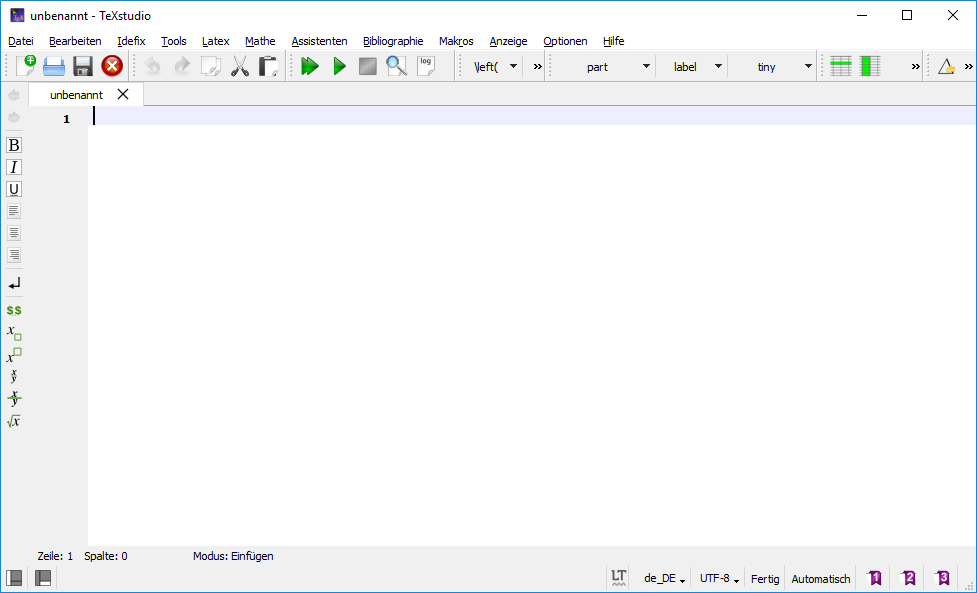
\includegraphics[keepaspectratio,width=12cm]{img/editor.png}};
		\draw (6,4) node[font=\huge]{?};
	\end{tikzpicture}
\end{center}
\end{frame}

\begin{frame}[t]{LaTeX-Vorlagen}
\begin{itemize}
	\item Das Erstellen einer eigenen Vorlage kostet viel Zeit und Nerven\dots
	\item<2-> Daher ist es vollkommen in Ordnung, auf bestehende Vorlagen zurückzugreifen.
	\item<3-> Im Learnweb stehen zwei Vorlagen für Übungszettelabgaben zu Verfügung.
	\begin{itemize}
		\item<4-> Wichtige Pakete und nützliche Befehle sind bereits eingerichtet.
		\item<5-> Racket- und Java-Quellcode kann mit Syntax Highlighting eingebunden werden.
		\item<6-> Präambel ist der Übersichtlichkeit halber in separate Datei \code{config.tex} ausgelagert.
		\item<7-> Kann beliebig angepasst werden.
	\end{itemize}
\end{itemize}
\end{frame}

\begin{frame}[t]{Hilfestellungen}
\begin{itemize}
	\item Suchmaschine eurer Wahl mit passenden (vorzugsweise englischen) Begriffen oder Ausgaben des Compilers füttern.
	\begin{center}
		
\includegraphics[keepaspectratio,width=8cm]{img/google.png}
	\end{center}
	\item<2-> LaTeX Stack Exchange: \url{https://tex.stackexchange.com}
	\item<3-> Im Diskussionsforum im Learnweb
	\begin{itemize}
		\item<4-> Fragen sollten hier möglichst konkret gestellt werden, etwa \enquote{Wie kann ich \dots \ bewerkstelligen?}, aber nicht \enquote{Kann jemand meinen Fehler suchen?}
	\end{itemize}
\end{itemize}
\end{frame}

\section*{Quellen}
\begin{frame}[allowframebreaks]{\secname}
	\printbibliography
\end{frame}


\end{document}